%--------------------------------------------CAPA DE IMPLEMENTACION Y MIGRACION ------------------------------------------------------%



\subsection{Capa de implementación y migración}
Los elementos de implementación y migración respaldan la implementación y migración de arquitecturas. Esto incluye modelar programas y proyectos de implementación para respaldar la gestión de programas, carteras y proyectos. También incluye \textbf{apoyo a la planificación migratoria.}
La Tabla \ref{tab:Tabla de la capa implementación y migración} ofrece una descripción general de los elementos de implementación y migración, con sus definiciones.\cite{archimate} 

\begin{longtable}{|p{0.15\linewidth}|p{0.45\linewidth}|p{0.2\linewidth} p{0.2\linewidth}|}
   \caption{Tabla de la capa implementación y migración}
   \\
   \hline
   \rowcolor[HTML]{AFC5F6} 
   \textbf{Elemento} & \textbf{Descripción} & \multicolumn{2}{c|}{\textbf{Notación}} \\
   \hline
   \endhead
   \hline
   \multicolumn{4}{r}{\textit{Continúa en la siguiente página}} \\
   \endfoot
   \hline
   \endlastfoot
   \label{tab:Tabla de la capa implementación y migración}
   %Contenido 1 &
   %\lipsum[1] &
   %Datos A1
   %& Datos B1
   %\\
   %\hline



   Paquete de trabajo 
   &
   Representa una serie de acciones identificadas y diseñadas para lograr resultados específicos dentro de limitaciones de tiempo y recursos específicas. 
   &
\begin{center}
   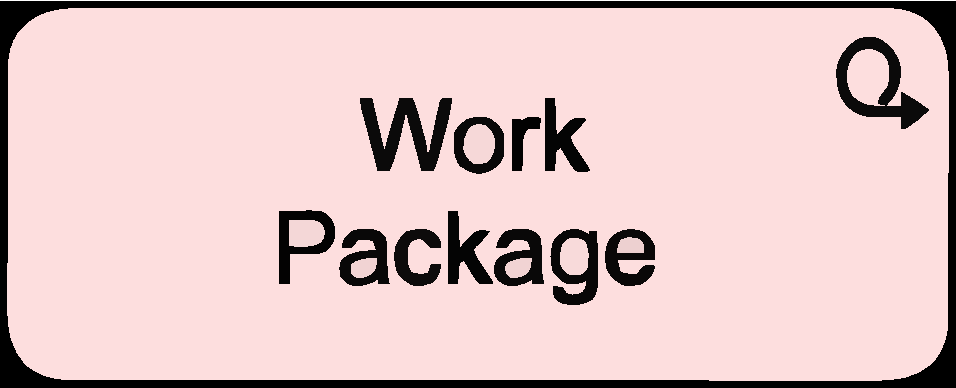
\includegraphics[width=1\linewidth]{imgs/capa_migracion/1.pdf}
\end{center} 
&
\begin{center}
   
\includegraphics[width=0.5\linewidth]{imgs/capa_migracion/a1.pdf}
\end{center}
   \\ \hline



   Entregable
   &
   Representa un resultado definido con precisión de un paquete de trabajo. 
   &
\begin{center}
   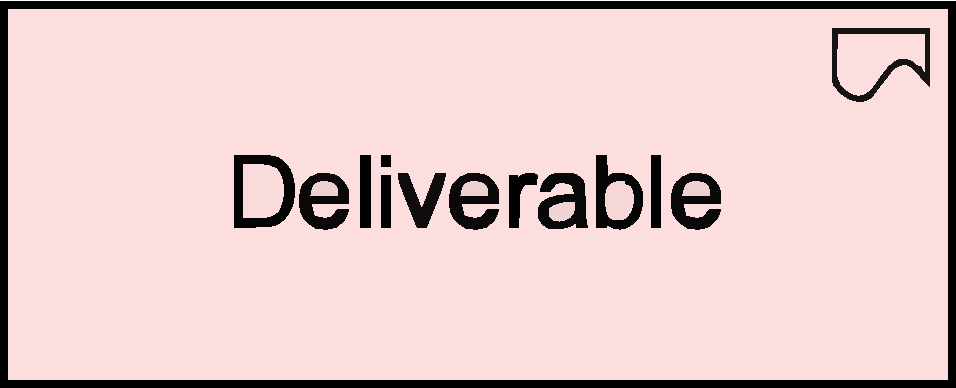
\includegraphics[width=1\linewidth]{imgs/capa_migracion/2.pdf}
\end{center} &
\begin{center}
   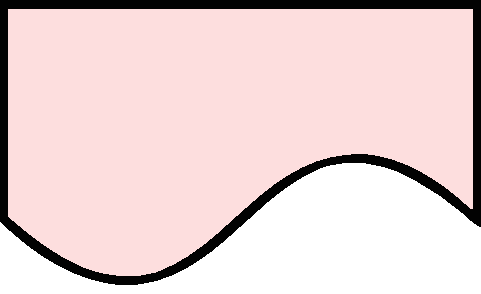
\includegraphics[width=0.5\linewidth]{imgs/capa_migracion/a2.pdf}
\end{center}
   \\ \hline



   Evento de implementación 
   &
   Representa un cambio de estado relacionado con la implementación o migración. 
   &
\begin{center}
   
\includegraphics[width=1\linewidth]{imgs/capa_migracion/3.pdf}
\end{center} &
\begin{center}
   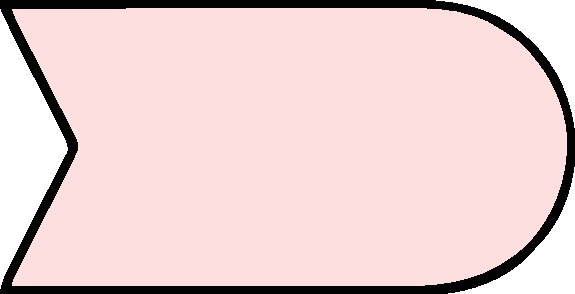
\includegraphics[width=0.5\linewidth]{imgs/capa_migracion/a3.pdf}
\end{center}
   \\ \hline



   Meseta
   &
   Representa un estado relativamente estable de la arquitectura que existe durante un período de tiempo limitado. 
   &
\begin{center}
   
\includegraphics[width=1\linewidth]{imgs/capa_migracion/4.pdf}
\end{center} &
\begin{center}
   
\includegraphics[width=0.5\linewidth]{imgs/capa_migracion/a4.pdf}
\end{center}
   \\ \hline

   Brecha
   &
   Representa una declaración de diferencia entre dos mesetas. 
   &
\begin{center}
   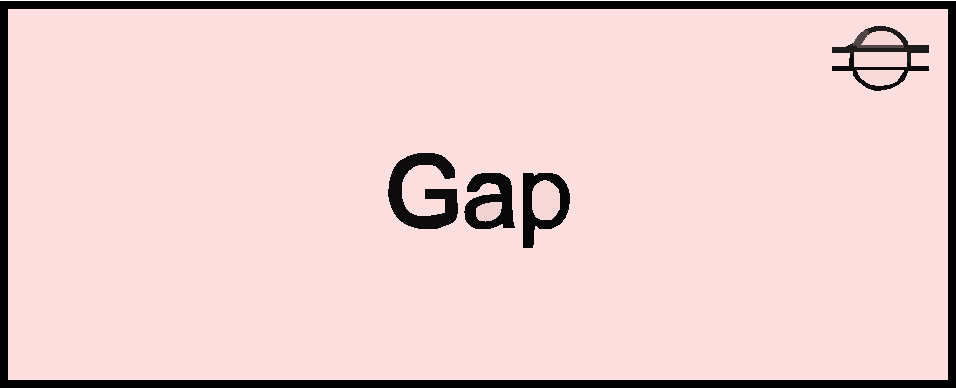
\includegraphics[width=1\linewidth]{imgs/capa_migracion/5.pdf}
\end{center} &
\begin{center}
   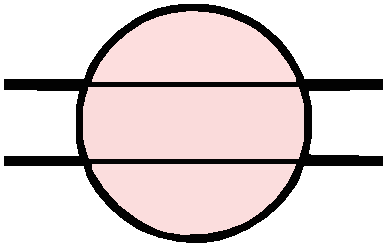
\includegraphics[width=0.5\linewidth]{imgs/capa_migracion/a5.pdf}
\end{center}
   \\ \hline

\end{longtable}
